% This is based on the LLNCS.DEM the demonstration file of
% the LaTeX macro package from Springer-Verlag
% for Lecture Notes in Computer Science,
% version 2.4 for LaTeX2e as of 16. April 2010
%
% See http://www.springer.com/computer/lncs/lncs+authors?SGWID=0-40209-0-0-0
% for the full guidelines.
%

\documentclass{llncs}

\usepackage[utf8]{inputenc}
\usepackage[T1]{fontenc}
\usepackage[polish]{babel}
\usepackage[colorinlistoftodos]{todonotes}
\usepackage{hyperref}
\usepackage{subfigure}
\usepackage[]{algorithm2e}
\usepackage[]{graphicx}
\usepackage{float}

\usepackage{listings}
\usepackage{courier}
 \lstset{
         basicstyle=\footnotesize\ttfamily,
         xleftmargin=.4\textwidth, xrightmargin=.2\textwidth
 }

\begin{document}

\title{Raport z testów rozwiązania problemu kajaków}
%
\titlerunning{Kajaki}  % abbreviated title (for running head)
%                                     also used for the TOC unless
%                                     \toctitle is used
%
\author{Tomasz Janiszewski\inst{1} \and Jakub Dutkowski\inst{2}}
%
\authorrunning{Tomasz Janiszewski, Jakub Dutkowski} % abbreviated author list (for running head)
%
%%%% list of authors for the TOC (use if author list has to be modified)
\tocauthor{Tomasz Janiszewski and Jakub Dutkowski}

\institute{Politechnika Warszawska\\
Wydział Matematyki i Nauk Informacyjnych
\email{janiszewskit@student.mini.pw.edu.pl}~~
\email{dutkowskij@student.mini.pw.edu.pl}}

\maketitle              % typeset the title of the contribution

\keywords{Kajaki}
%
\section{Wstęp}
W celu zbadania poprawności działania programu, przeprowadziliśmy testy na następujących zestawach danych:
\begin{enumerate}
\item dane przypadkowe
\item dane przypadkowe
\item dane, w których jedna liczba jest zawarta w każdej parze wejściowej
\item dane, w których graf par wejściowych jest cyklem
\end{enumerate}

\section{Treść zadania}
Są dwa kajaki, $n$ osób i zbiór par osób które chcą się
przepłynać kajakiem razem (jedna osoba może kolejno z wieloma osobami się
przepłynać). Zastosować algorytm znajdujący skojarzenie doskonałe do
wyznaczenia rozkładu jazdy kajaków, tak aby zminimalizować ilość kursów
pojedynczym kajakiem, spełniając życzenia wszystkich osób.

\section{Wyniki testów}
\subsection{Zestaw 1.}
\begin{example} \label{Zestaw1} ~\\
\begin{lstlisting}[title=Wejście]
6 7
1 2
1 6
2 3
2 6
3 5
4 5
5 6
\end{lstlisting}
\begin{lstlisting}[title=Wyjście]
(1, 2), (5, 6)
(2, 6), (3, 5)
(6, 7), (2, 3)
(4, 5), (1, 6)
\end{lstlisting}
\end{example}

\section{Wyniki testów}
\subsection{Zestaw 2.}
\begin{example} \label{Zestaw2} ~\\
\begin{lstlisting}[title=Wejście]
1 2
3 4
3 2
3 6
3 5
1 7
7 3
\end{lstlisting}
\begin{lstlisting}[title=Wyjście]
(1, 2), (3, 5)
(1, 7), (3, 4)
(2, 3), ()
(3, 6), ()
(3, 7), ()
\end{lstlisting}
\end{example}

\subsection{Zestaw 3.}
\begin{example} \label{Zestaw3} ~\\
\begin{lstlisting}[title=Wejście]
1 7
1 2
1 6
1 3
1 4
1 5
1 8
1 9	
\end{lstlisting}
\begin{lstlisting}[title=Wyjście]
(1, 2), ()
(1, 3), ()
(1, 4), ()
(1, 5), ()
(1, 8), ()
(1, 6), ()
(1, 9), ()
(1, 7), ()
\end{lstlisting}
\end{example}

\subsection{Zestaw 4.}
\begin{example} \label{Zestaw4} ~\\
\begin{lstlisting}[title=Wejście]
1 2
2 3
3 4
5 6
6 7
7 8
8 1
\end{lstlisting}
\begin{lstlisting}[title=Wyjście]
(1, 2), (7, 8)
(5, 6), (2, 3)
(1, 8), (3, 4)
(6, 7), ()
\end{lstlisting}
\end{example}

\section{Opis wyników}
W każdym z przedstawionych przypadków program działał poprawnie. 

\subsection{Zestaw 1}
W zestawie nr 1 wszystkie wymagania zostały spełnione już w czterech rundach, w każdej rundzie oba kajaki są wypełnione, więc nie istnieje lepsze rozwiązanie.

\subsection{Zestaw 2}
W zestawie nr 2 aż 5 par zawiera liczbę 3, stąd wiadomo że najlepsze rozwiązanie nie może być mniejsze niż 5 rund. Zostało znalezione właśnie takie rozwiązanie i jest ono zgodne z warunkami zadania, stąd wiadomo że algorytm zadziałał poprawnie.

\subsection{Zestaw 3}
Zestaw 3 jest przypadkiem szczególnym, w którym jedna z liczb występuje w dokładnie każdej parze, stąd wiadomo że nie może istnieć rozwiązanie lepsze niż znalezione przez algorytm. Oczywiście widać, że znalezione rozwiązanie jest poprawne

\subsection{Zestaw 4}
Zestaw 4 jest przypadkiem szczególnym, w którym graf rozkładu pływania zawiera cykl. Widać i tutaj, że rozwiązanie krótsze nie istnieje, a znalezione jest poprawne.

\section{Opracowanie złożoności}
W celu sprawdzenia poprawności wyznaczonej teoretycznie złożoności algorytmu
\begin{equation}
O(|V|^6)
\end{equation}
Przeprowadzono testy, w których dla liczby wierchołków ($|V|$) kolejno $[5, 10, 15, 20, 25, 30, 35, 40, 45, 50]$ i liczby krawędzi ($|E|$) równej $|E|=\alpha\times|V|$, dla $\alpha$ kolejno $[0.25, 0.50, 0.75, 1.0]$ generowano grafy losowe. 

Na wykresach \autoref{fig:complexity} przedstawiono zależność znormalizowanego czasu wykonania algorytmu od liczby wierzchołków dla różnych $\alpha$. Do wyliczonych punktów dopasowano krzywą $f(x) = a\times x^6 + b$. Przedstawione wartości są średnią z 50 pomiarów wykonanych dla każdej wartości parametrów.

Z wykresów można wnioskować, że wyznaczona złożoność pokrywa się z wartościami empirycznymi. Lepsze dopasowanie dla dużych wartości $\alpha$ może wynikać z oszacowania liczby krawędzi przez graf pełny w wyliczeniach teoretycznych.

\begin{figure}
\centering
\begin{subfigure}
  \centering
  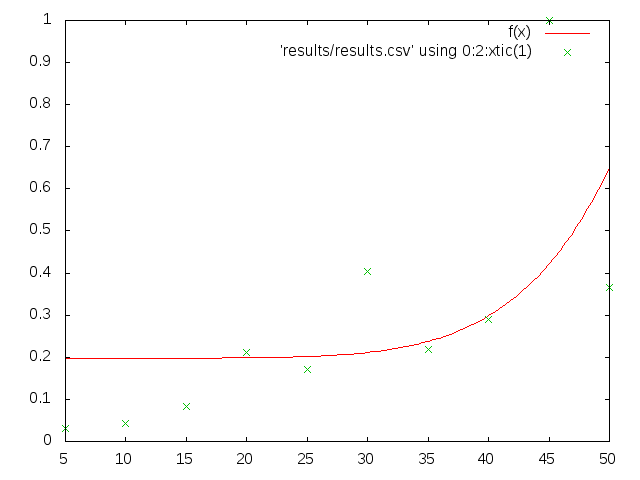
\includegraphics[width=.4\linewidth]{img/25.png}
  \caption{$\alpha=0.25$}
  \label{fig:sub1}
\end{subfigure}%
\begin{subfigure}
  \centering
  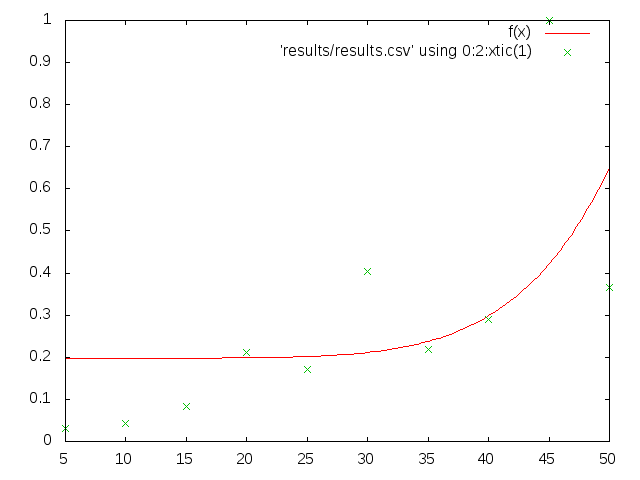
\includegraphics[width=.4\linewidth]{img/50.png}
  \caption{$\alpha=0.50$}
  \label{fig:sub2}
\end{subfigure}
%
\begin{subfigure}
  \centering
  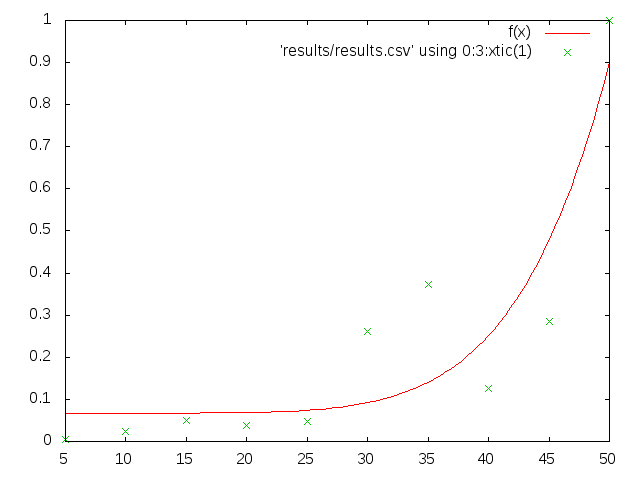
\includegraphics[width=.4\linewidth]{img/75.png}
  \caption{$\alpha=0.75$}
  \label{fig:sub2}
\end{subfigure}
%
\begin{subfigure}
  \centering
  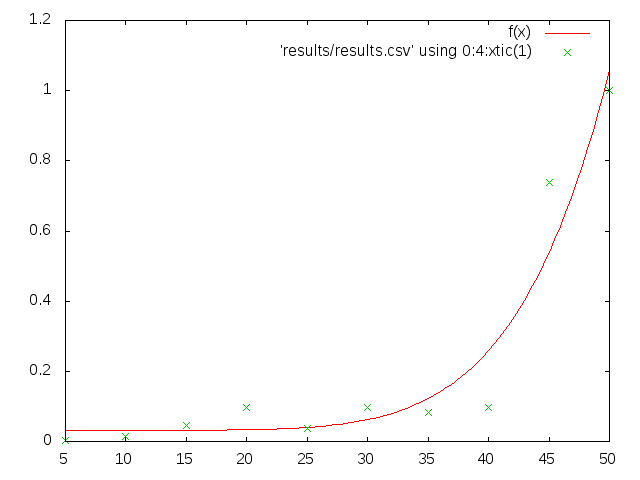
\includegraphics[width=.4\linewidth]{img/100.png}
  \caption{$\alpha=1.00$}
  \label{fig:sub2}
\end{subfigure}
%
\begin{subfigure}
  \centering
  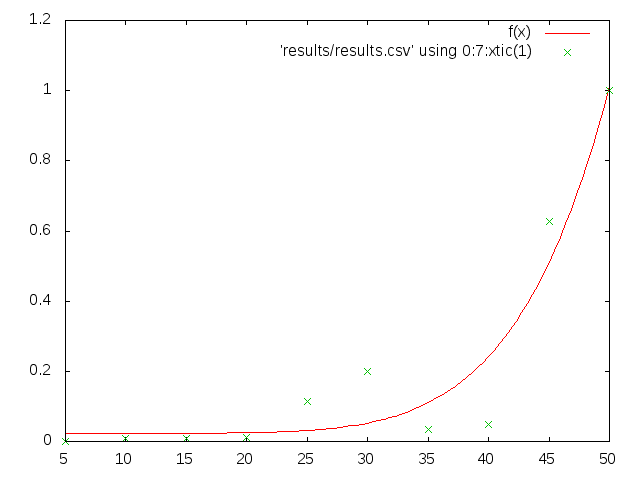
\includegraphics[width=.4\linewidth]{img/150.png}
  \caption{$\alpha=1.50$}
  \label{fig:sub2}
\end{subfigure}
\caption{Wykresy zależności znormalizowanego czasu wykonania od liczby krawędzi}
\label{fig:complexity}
\end{figure}

\section{Wnioski}
W raporcie przedstawione zostały niektóre przypadki na których testowane było rozwiązanie zadania przedstawiające zarówno dane przypadkowe jak i wybrane w sposób szczególny.

W testach nie znaleziono przypadków, dla których algorytm zadziałał by źle, więc można wnioskować, że implementacja jest poprawna.

% ---- Bibliography ----
%
\begin{thebibliography}{4}
%
\bibitem {cormen}
Cormen, Thomas H. and Stein, Clifford and Rivest, Ronald L. and Leiserson, Charles E.:
\textsl{Introduction to Algorithms}
McGraw-Hill Higher Education, 2001
\bibitem{mucha-sankowski}
Mucha, Marcin and Sankowski, Piotr:
\textsl{\href{http://www.mimuw.edu.pl/~mucha/pub/mucha_sankowski_focs04.pdf}{Maximum Matchings via Gaussian Elimination}}
\bibitem{wiki-blossom}
Wikipedia:
\textsl{\href{http://en.wikipedia.org/wiki/Blossom_algorithm}{Edmonds's matching algorithm}}
\end{thebibliography}

\end{document}
